\documentclass[11pt,letterpaper]{article}

%\usepackage[latin1]{inputenc} 
\usepackage[utf8]{inputenc}
\usepackage[cyr]{aeguill}
\usepackage[colorlinks=true]{hyperref}
\usepackage{textpos}
\usepackage{graphicx}
\usepackage[french]{babel}
\usepackage{color}
\usepackage{array}
\usepackage{enumerate}
\usepackage{fancyhdr}
\usepackage{lastpage}
\usepackage{amsmath}
\usepackage{amssymb}
\usepackage{epstopdf}
\usepackage{mathrsfs}
\usepackage{float}
\usepackage{multicol}
\usepackage{caption}
\usepackage{subcaption}
\usepackage{siunitx}
\addto\captionsfrench{\def\tablename{Tableau}}

%-----------------------------------------------------------------%
% Definitions
\newcommand{\session}{Hiver 2022}
\newcommand{\firstauthor}{Yoan \textbf{Fournier}}
\newcommand{\firstregistrationnumber}{1958736}
\newcommand{\secondauthor}{Victor \textbf{Gaudreau-Blouin}}
\newcommand{\secondregistrationnumber}{1958297}
\newcommand{\reportnumber}{}
\newcommand{\firsttitle}{Analyse énergétique d'un processeur vectoriel pour des calculs de DNN}
\newcommand{\secondtitle}{Rapport intermédiaire}
%-----------------------------------------------------------------%



\oddsidemargin 0pt
\topmargin 0pt
\textwidth 6.5in
\textheight 8.1in

\setlength{\parskip}{1em}

\definecolor{bleu_poly}{RGB}{65,170,230}
\definecolor{vert_poly}{RGB}{140,200,60}
\definecolor{orange_poly}{RGB}{250,150,30}
\definecolor{rouge_poly}{RGB}{185,30,50}
\definecolor{gris_poly}{RGB}{166,168,171}


\title{\vspace{-2.5cm} \noindent\makebox[\linewidth]{\color{rouge_poly}{\rule{\textwidth}{1.5pt}}}
        \begin{center}
        \begin{tabular}{m{6.5cm}m{6cm}}
        \textbf{ \huge Projet \reportnumber}  & 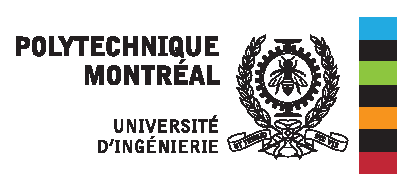
\includegraphics[width=0.4\textwidth]{Polytechnique_signature-CMYK-droite_FR.eps}
        \end{tabular}
        \end{center}
        \noindent\makebox[\linewidth]{\color{rouge_poly}{\rule{\textwidth}{1.5pt}}}
        \\ \  \\
        \Huge \firsttitle \\ \secondtitle  
        \\ \ \\
        \LARGE ELE6307 - Machines neuronales : architectures et applications
        }

\author{\session \\ Département de génie électrique \\ École Polytechnique de Montréal} 

\date{Dernière mise à jour: \today}

\pagestyle{fancy}

\lfoot{\session}
\cfoot{ELE6307 - Machines neuronales : architectures et applications}
\rfoot{\thepage/\pageref{LastPage}}
\chead{}
\lhead{\emph{Projet -- \firstauthor  \, (\firstregistrationnumber)/\secondauthor\,  (\secondregistrationnumber)}}
\rhead{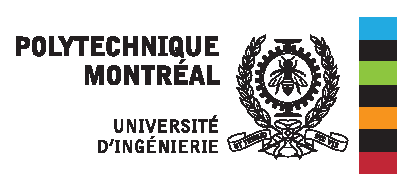
\includegraphics[width=2.5cm]{Polytechnique_signature-CMYK-droite_FR.eps}}
\renewcommand{\headrulewidth}{0.4pt}
\renewcommand{\footrulewidth}{0.4pt} 
\setlength{\headheight}{45pt}


\graphicspath{{fig/}}


\newcommand{\vb}[1]{\mathbf{#1}}
\newcommand{\bs}[1]{\boldsymbol{#1}}


%-----------------------------------------------------------------%
% SOF
\begin{document}
\maketitle
\noindent\makebox[\linewidth]{\color{rouge_poly}{\rule{\textwidth}{1.5pt}}} 


\noindent \LARGE \firstauthor  \hfill \firstregistrationnumber


\noindent \LARGE \secondauthor \hfill \secondregistrationnumber


\noindent\makebox[\linewidth]{\color{rouge_poly}{\rule{\textwidth}{1.5pt}}}


\newpage
\normalsize

\section*{Introduction}
    \begin{multicols}{2}
    Afin de modéliser l'efficacité énergétique du coprocesseur vectoriel ARA, le simulateur Timeloop a été 
    utilisé. Ce simulateur utilise une structure hiérarchique pour modéliser une architecture. Une structure
    détaillant le problème à résoudre par l'architecture est aussi spécifiée. La commande \textit{timeloop-mapper}
    permet ensuite de trouver automatiquement la correspondance idéale du problème sur l'architecture matérielle.

    L'architecture simplifiée de ARA, comme mentionnée dans la proposition du projet, peut se modéliser en termes de 
    \textit{Lanes}. Chaque \textit{Lanes} à sa plus simple expression consiste en une banque de 8 registres ainsi qu'une
    unité arithmétique capable d'effectuer des multiplications et des additions. Bien que sur ARA, l'unité d'addition 
    est séparée de l'unité de multiplication, les deux unités peuvent fonctionner durant le même cycle sur des données
    indépendantes. Dans le cadre de la modélisation, on simplifie en utilisant la structure \textit{intmac} fournie par
    l'outil Timeloop-Accelergy. Nous considérons que la différence causée par cette simplification est minimale. En effet,
    les opérations dans une Lane sont pipelinées et les opérations de multiplication et addition peuvent être exécutées en même temps.
    La seule différence principale est la latence causée par le pipelinage des opérations. Cependant, ce n'est pas une métrique
    de performance étudiée dans le cadre de ce projet.

    L'architecture utilisée est présentée à la figure \ref{fig:arch}. On y observe une mémoire DRAM principale reliée à 
    la mémoire cache L1 de 64 KB. La cache L1 est reliée à un nombre paramétrable de \textit{Lanes}. 
    Chaque \text{Lane} comporte sa banque de 8 registres et son unité de \text{multiply-accumulate}.

    \begin{figure}[H]
        \centering
        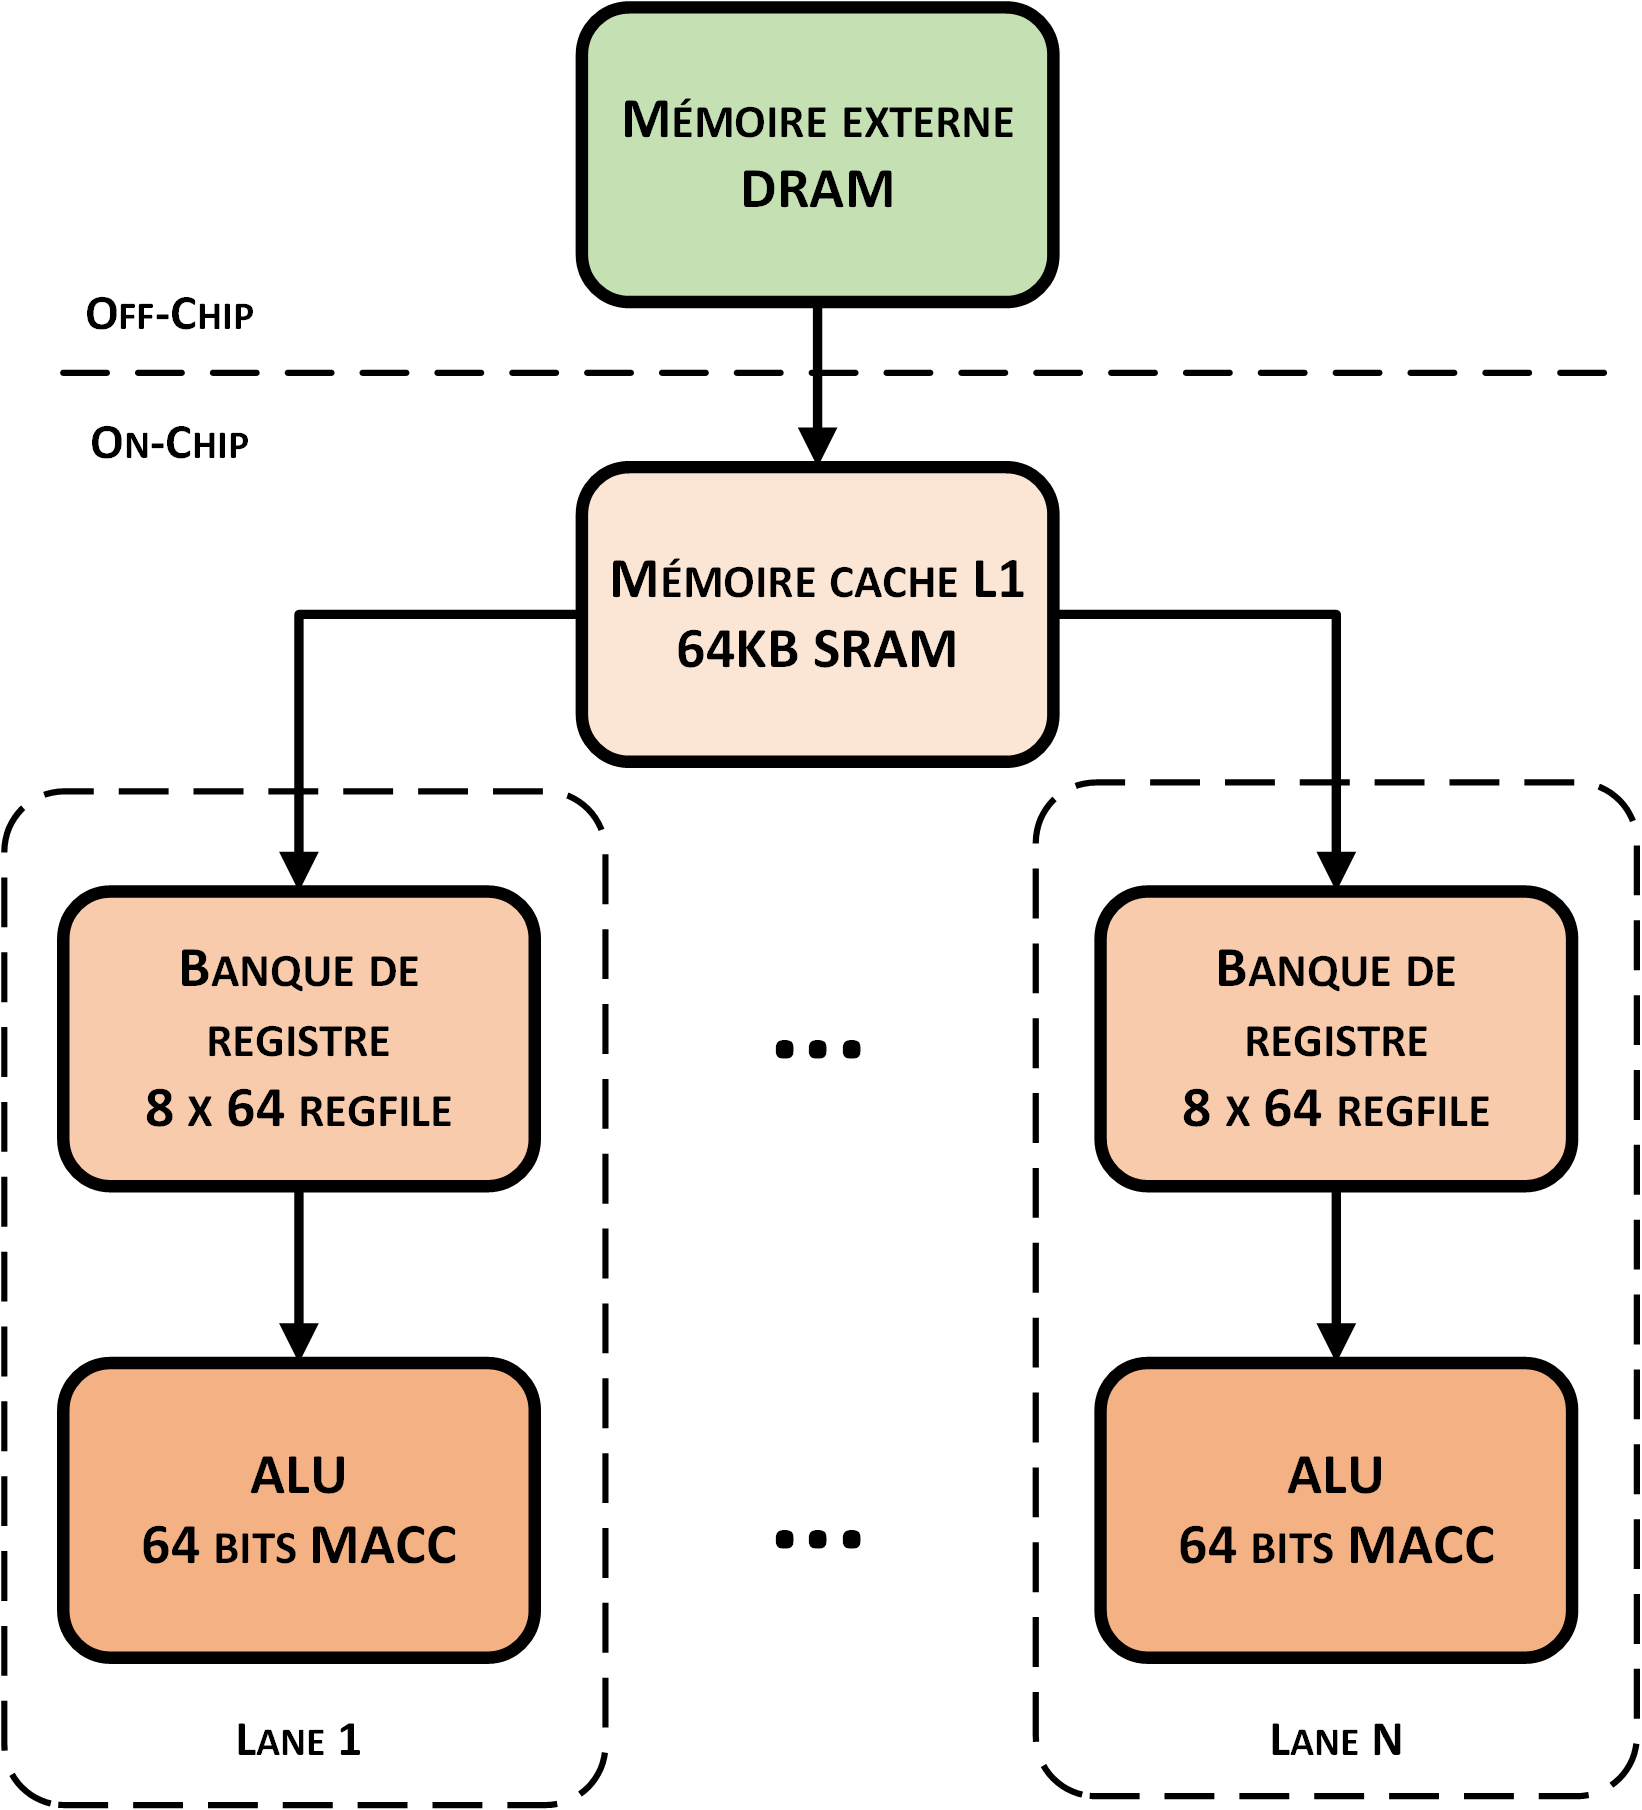
\includegraphics[width=\linewidth]{arch_visio.png}
        \caption{Architecture de ARA sur Timeloop}
        \label{fig:arch}
    \end{figure}

    Afin d'étudier la performance de l'architecture en fonction du nombre de \textit{Lanes}, le problème utilisé est la première 
    couche convolutionnelle du modèle VGG16. Cette couche comporte 64 filtres avec un \textit{kernel} de $3\times3$. L'entrée de la couche
    est une image de dimension $224\times224\times3$.  

    \end{multicols}


\pagebreak
\section*{Résultats}
    % TODO: Performance GFLOP/W 
    % TODO: Area (45nm + 22nm)
    \begin{multicols}{2}
        
    \begin{figure}[H]
        \centering
        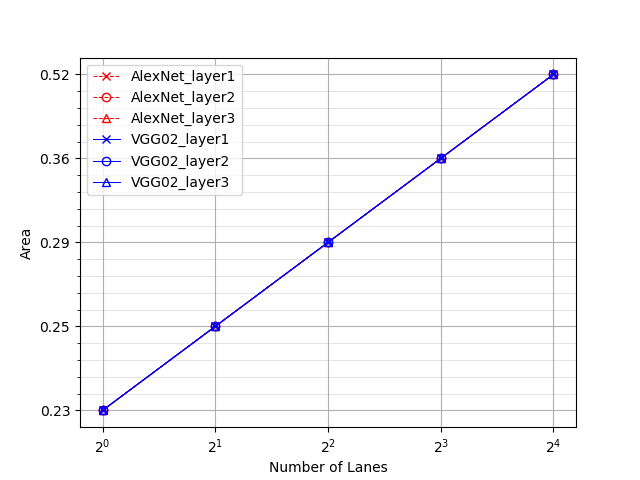
\includegraphics[width=\linewidth]{area.png}
        \caption{Aire de ARA en fonction du nombre de \textit{Lanes} pour la couche 1 de VGG16}
        \label{fig:area}
    \end{figure}
    \begin{figure}[H]
        \centering
        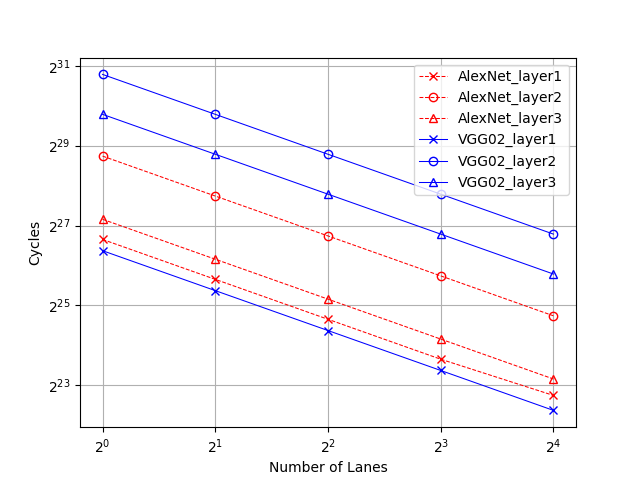
\includegraphics[width=\linewidth]{cycles.png}
        \caption{Cycles de ARA en fonction du nombre de \textit{Lanes} pour la couche 1 de VGG16}
        \label{fig:cycles}
    \end{figure}
    \begin{figure}[H]
        \centering
        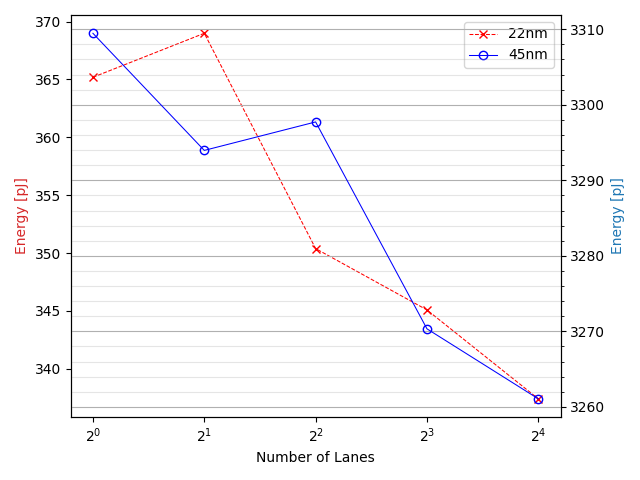
\includegraphics[width=\linewidth]{energy.png}
        \caption{Énergie de ARA en fonction du nombre de \textit{Lanes} pour la couche 1 de VGG16}
        \label{fig:energy}
    \end{figure}
    \begin{figure}[H]
        \centering
        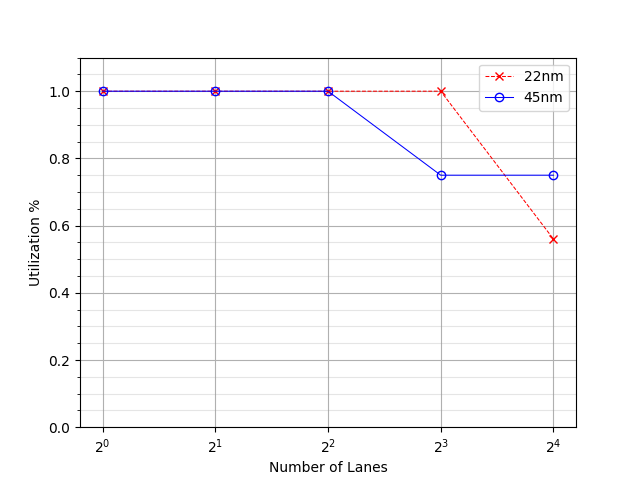
\includegraphics[width=\linewidth]{utilization.png}
        \caption{Utilisation de ARA en fonction du nombre de \textit{Lanes} pour la couche 1 de VGG16}
        \label{fig:utilization}
    \end{figure}


    \end{multicols}


\section*{Suite du projet}
    % TODO: Modélisation de la cache
    % TODO: Améliorer mapping pour 8 et 16 lanes
    % TODO: Tester pour différents paramètres de problèmes (Différentes convolutions)


\end{document} 
%-----------------------------------------------------------------%
% EOF